\documentclass[../slides.tex]{subfiles}
\begin{document}

\begin{frame}{Stitching: Grundlagen}
    \begin{minipage}[t]{.5\textwidth}
        \begin{itemize}
            \item Überlappender Bereich
            \item Features in beiden Bildern erkennen
            \item Features übereinanderlegen
            \item Konturen extrahieren
            \item Konturen transformieren
            \item Beste Überlappung berechnen
            \item Bild mit Transformation der besten Überlappung transformieren
            \item Beide Bilder zusammenfügen
        \end{itemize}
        \end{minipage}
        \hfill
        \begin{minipage}[t]{.45\textwidth}
        \begin{figure}[]
            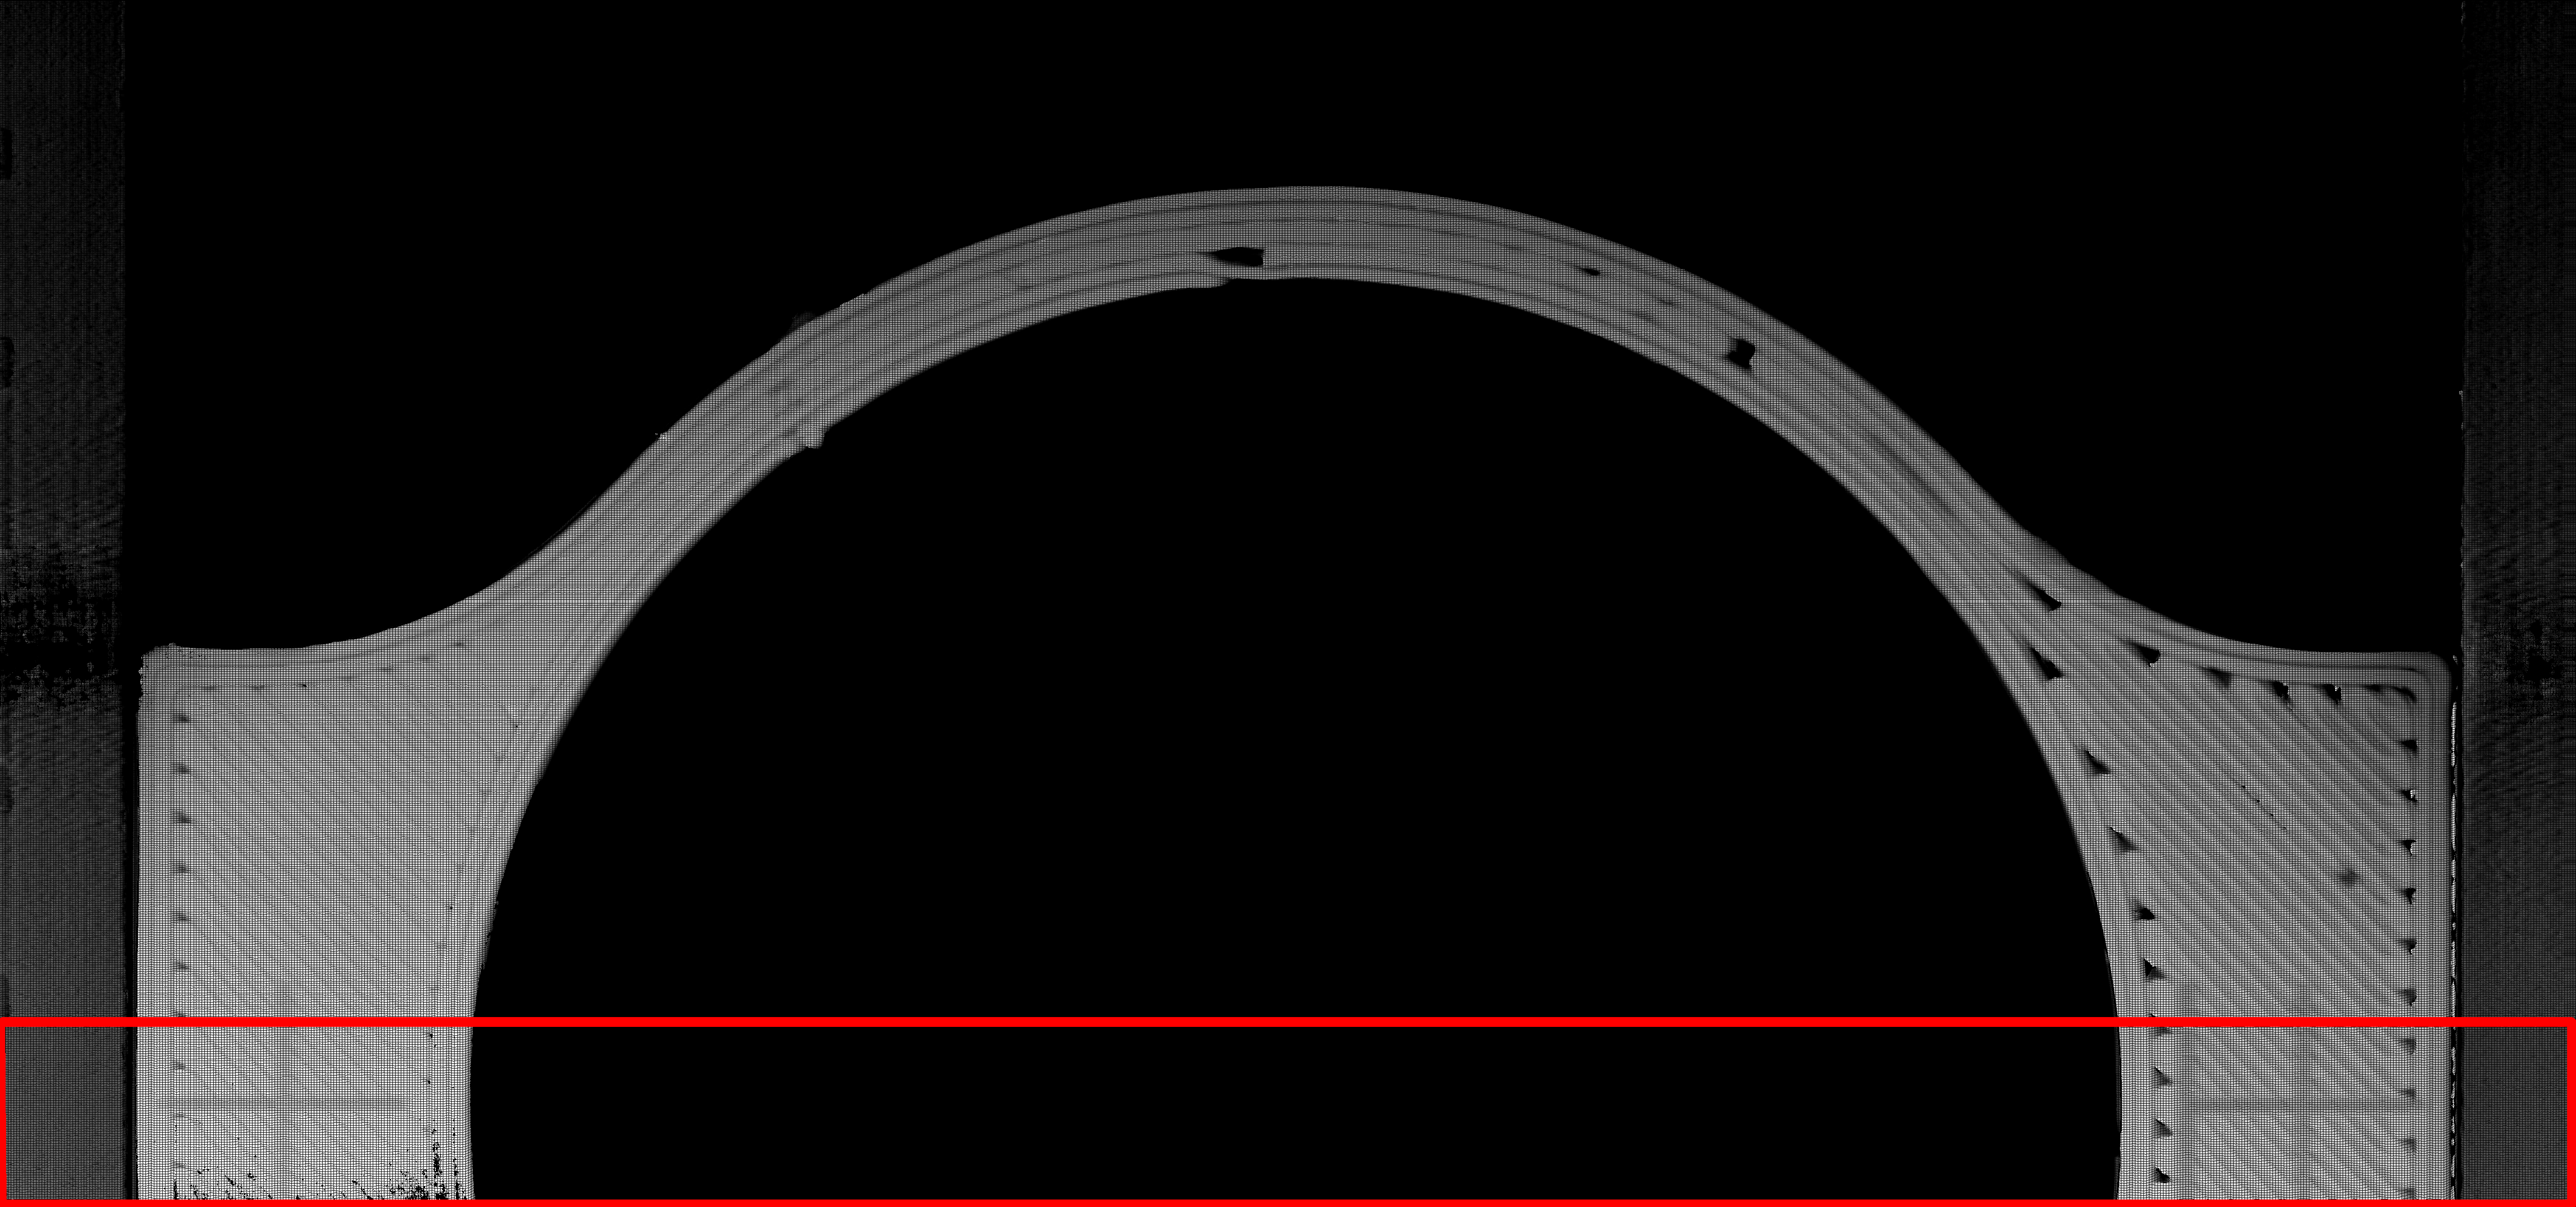
\includegraphics[angle=90, height=175pt]{img_niklas/fdm_top_10p_red.png}
            \caption{überlappender Bereich}
            \label{fig:versuchsaufbau}
        \end{figure}
        \end{minipage}
\end{frame}

\begin{frame}{Stitching: Konturen extrahieren}
    \begin{figure}
        \centering
        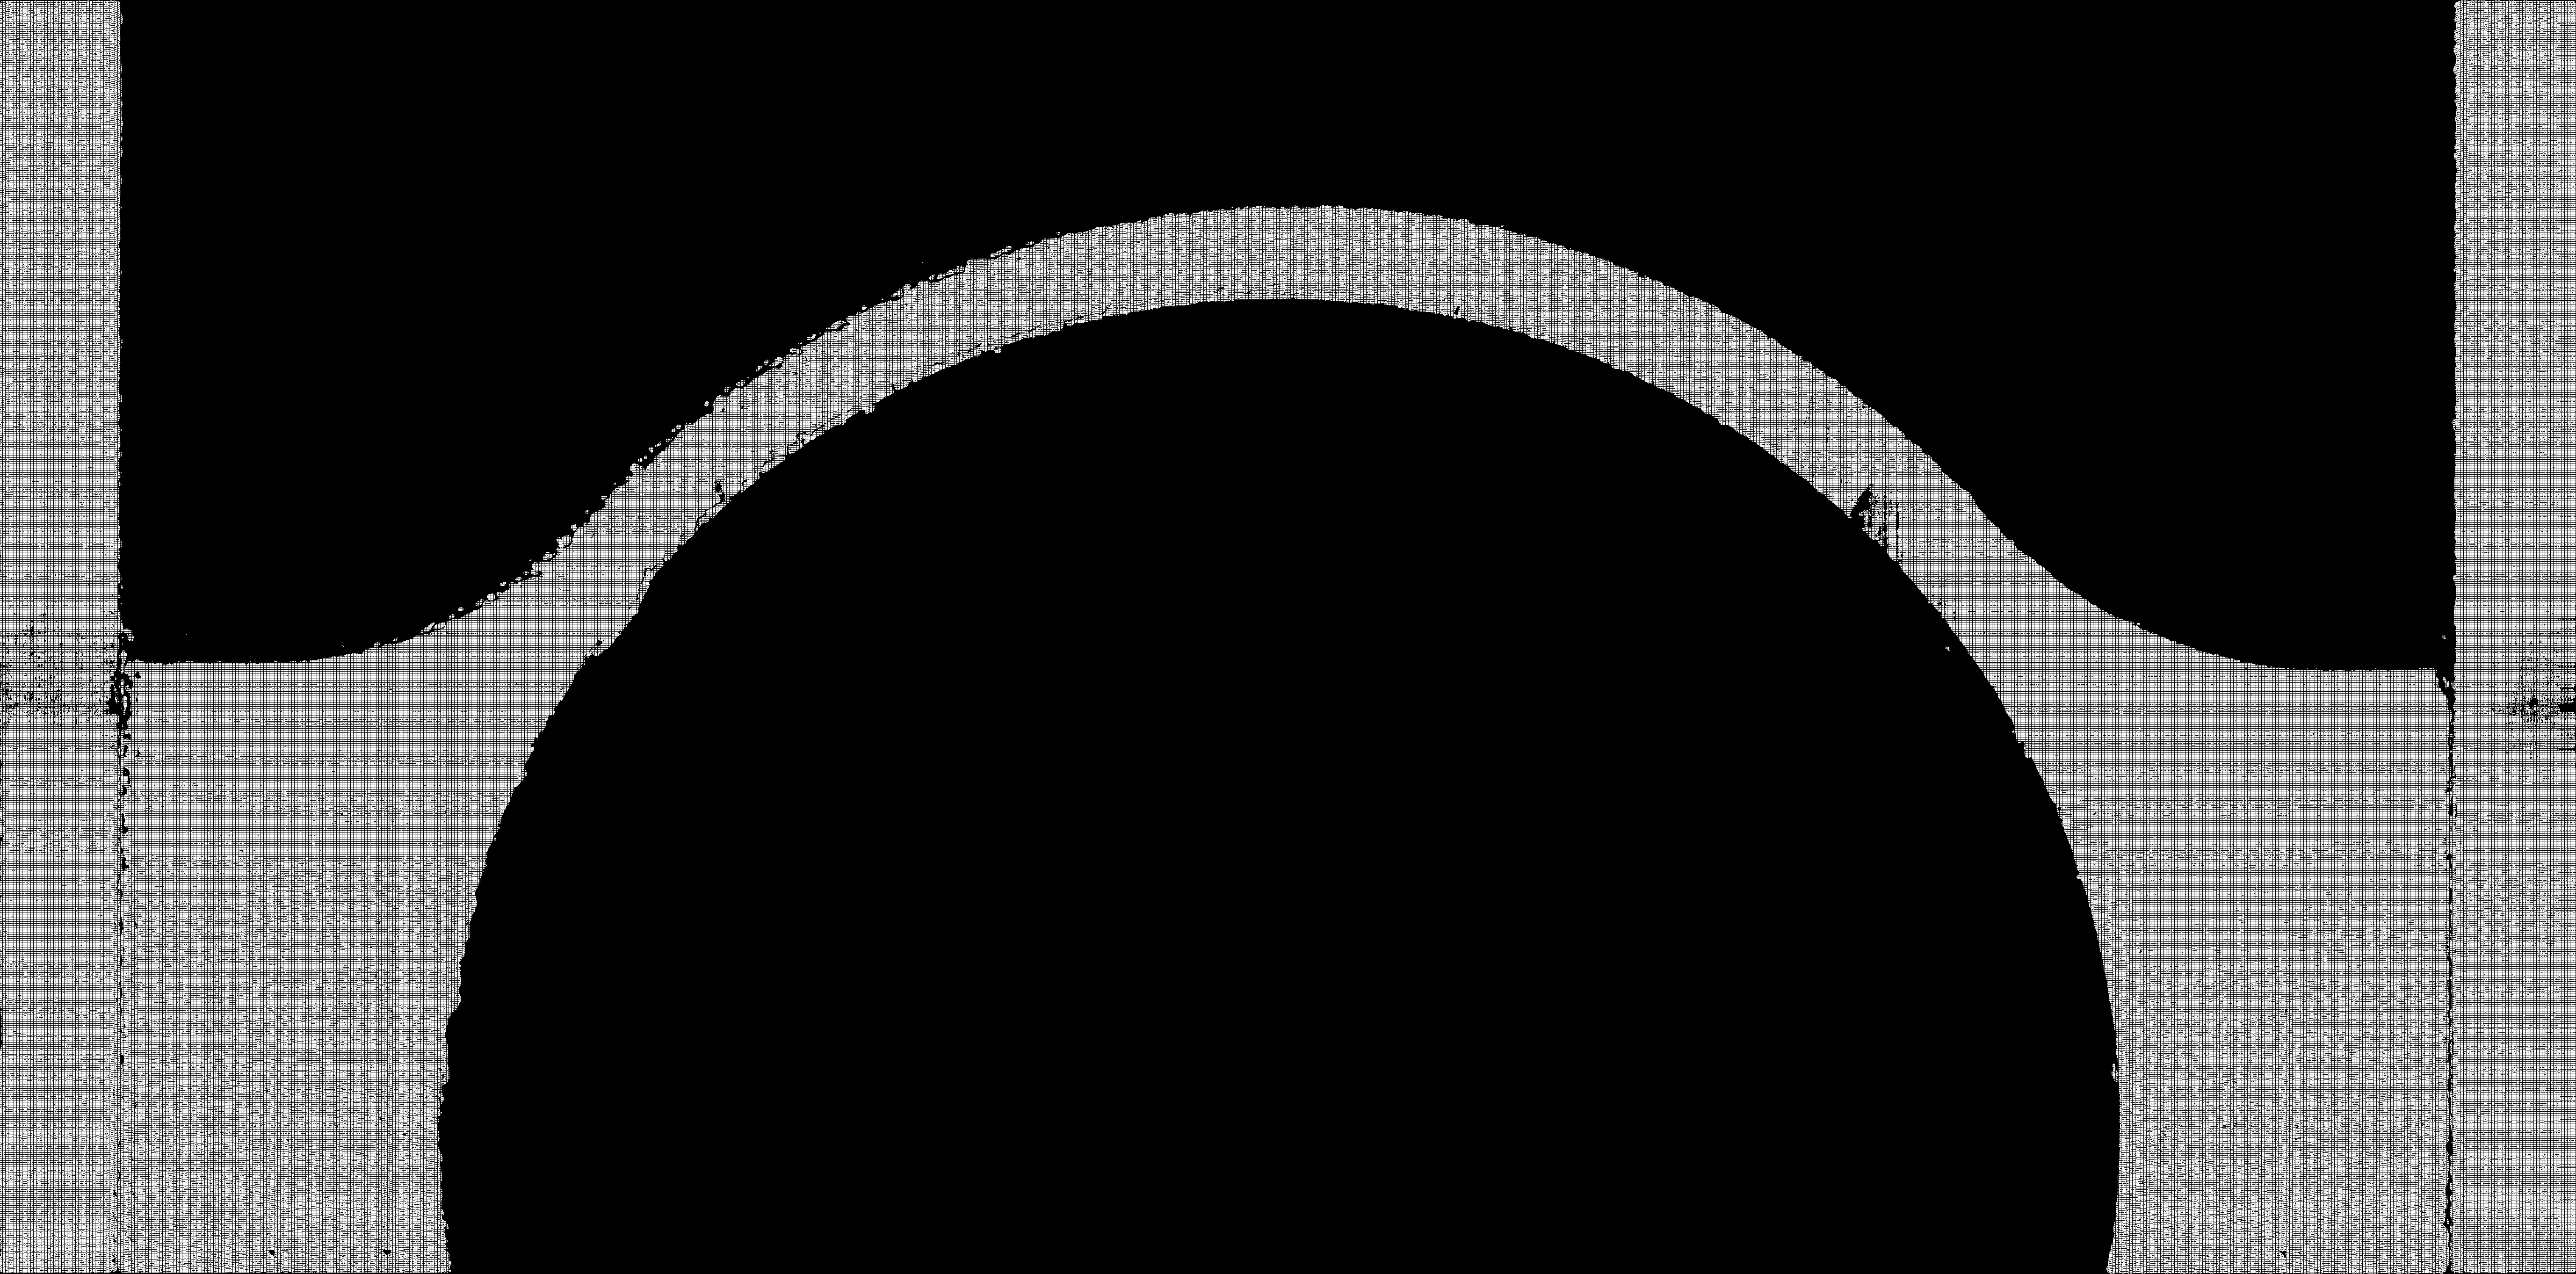
\includegraphics[height=175pt]{img_niklas/top.png}
        \caption{Bild eines Metallbauteil-Scan}
        \label{fig:ampic}
    \end{figure}
\end{frame}

\begin{frame}{Stitching: Konturen extrahieren}
    \begin{figure}
        \centering
        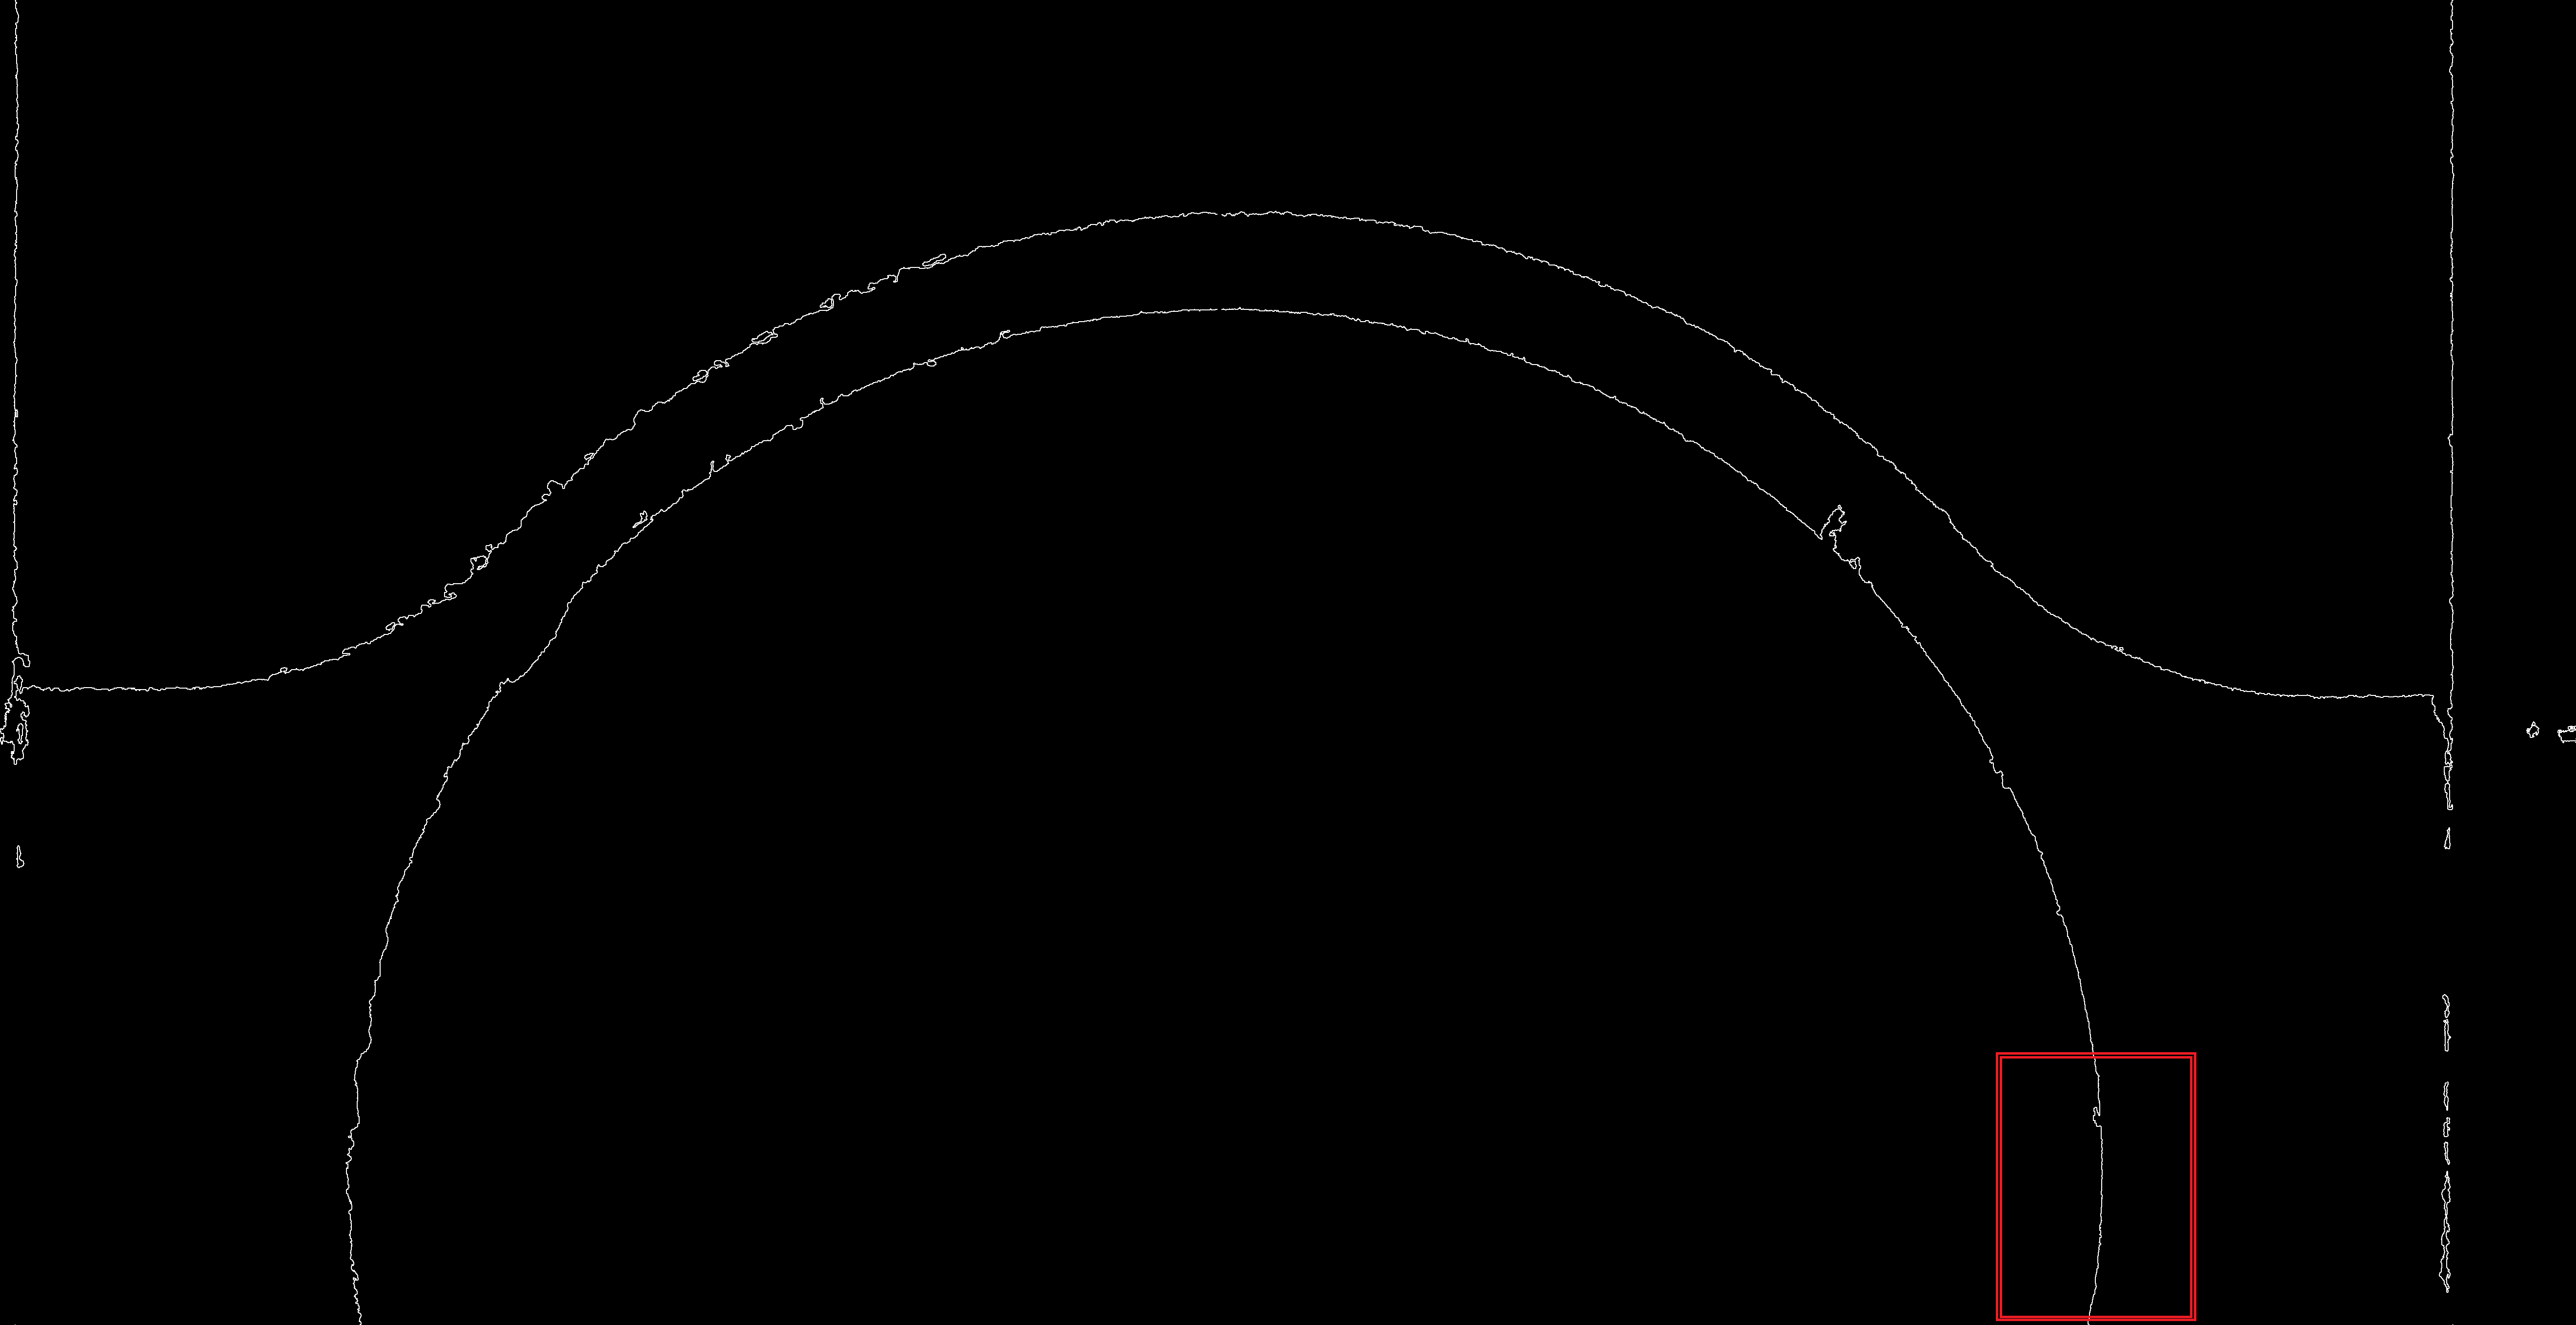
\includegraphics[height=175pt]{img_niklas/all_cons_top_red.png}
        \caption{Extrahierte Konturen}
        \label{fig:cons}
    \end{figure}
\end{frame}

\begin{frame}{Stitching: Konturen extrahieren}
    \centering
    \begin{minipage}[H]{.2\textwidth}
        \centering
        
\includegraphics[width=\textwidth]{img_niklas/0_match.png}
    \end{minipage}
    \begin{minipage}[H]{.15\textwidth}
        \centering
        
\includegraphics[width=\textwidth]{img_niklas/15_match.png}
    \end{minipage}
    \begin{minipage}[H]{.2\textwidth}
        \centering
        
\includegraphics[width=\textwidth]{img_niklas/382_match.png}
    \end{minipage}
    \begin{minipage}[H]{.2\textwidth}
        \centering
        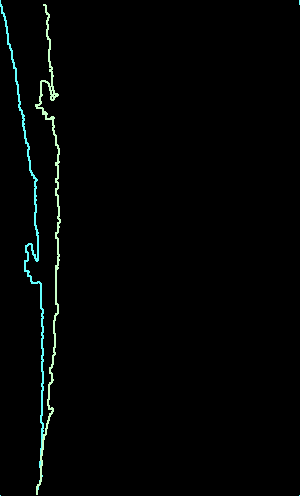
\includegraphics[width=\textwidth]{img_niklas/570_match.png}
    \end{minipage}

\end{frame}

\begin{frame}{Stitching: Resultat}
    \begin{figure}
        \centering
        
\includegraphics[height=175pt]{img_niklas/am_sp0_stitched_2.png}
        \caption{Stitching: Resultat}
        \label{fig:cons}
    \end{figure}
\end{frame}

\end{document}